\documentclass{article}
\usepackage[utf8]{inputenc}
\usepackage{natbib}
\usepackage{graphicx}
\usepackage{geometry}
\geometry{ margin=1.3in}
\usepackage{hyperref}
\usepackage{color}
\usepackage[table,xcdraw]{xcolor}
\usepackage{longtable}
\renewcommand\thesubsection{\alph{subsection}}
\usepackage{tabularx}
\usepackage{float}
\usepackage[T1]{fontenc}
\usepackage[USenglish]{babel}
\usepackage[nodayofweek,level]{datetime}
\newcommand{\mydate}{\formatdate{17}{10}{2017}}

\begin{document}
	\title{Requirement Documentation for MECH-APEX ZERO}
	\author{Tian Guo \and Yicheng Chen \and Jonathan Yu \and Yanting Zhang \and Saim Zahid}
	\selectlanguage{USenglish}
	\date{\mydate}
	\maketitle
	\newpage
	\tableofcontents
	
	\section{Purpose of the Project}
	The purpose of this project is to produce the game designed by the team: Mech-APEX Zero. Mech-APEX Zero is the combination of classical 2D games like Metroid, Castlevania, and Street Fighter. This game will reinvigorate the love for such classics and the modern spin of new combat mechanics will attract new players.
	
	\subsection{Background}
	The concept of this game was conceived to revitalize a very saturated genre of video games: Platformer. Currently on Steam, new releases of the Platformer Genre has 1167 results. The motivation of the team is to make a game that would stand out amongst the over one thousand competitors. In order to achieve our goal, we have examined the classics and commercial successes to create our project.
	
	\subsection{Goals}
	The goals of Team Chicken Sausage is to produce an entertaining game to satisfies the needs of our clients. We want our audience to get the enjoyment of playing a platformer and to be dazzled and surprised by our creative story and universe.
	
	\section{Stakeholders}
	\subsection{Development Team} Chicken and Sausages. 
	\subsection{Instructor} Dr. Jacques Carette  
	\subsection{Game Critics}
	\begin{itemize}
		\item Dr. Jacques Carette
		\item Daniel Szymczak
	\end{itemize}
	\subsection{Player} The players who enjoy platformers and beat em up games. 
	
	\section{Mandated Constraints}
	The game must have a certain degree of complexity attached to it, as required from Dr. Carrete, to gauge the students game development abilities better. This complexity goes hand in hand with the difficulty of developing the game as it is very easy to make tic tac toe compared to a game such as Skyrim. 
	
	\subsection{Solution Constraints}
	Project must use Unity Game Engine to develop the game. The main programming language used will be C\#. 
	
	\subsection{Implementation Environment of the Current System}
	The final product will be able to run on Windows, Mac OS, and Linux systems, as the Unity library allows to build project for all three platforms.
	Due to the nature of the game being a combo focused action platformer, control methods such as mouse control or touch screen will not be ideal. The development team will focus its effort on establishing keyboard as the main method of controls. Controllers such as Dualshock 4 and Xbox Controller are options, but do not have plans to implement these currently.
	
	\subsection{Partner or Collaborative Applications}
	The product of this project will comply with all policies of the Unity Free User's Licence Agreement.
	This product will not be used for commercial purposes as the assets used were of other Games.
	
	\subsection{Off-the-Shelf Software}
	Some assets used in this project is created through the use of GIMP. The final product shall comply with GIMP's user agreement.
	
	\subsection{Schedule Constraints}
	The deadline of the Project must be within the 2017-2018 Capstone Course terms. Revision 0 of the product must be completed by December of 2017.
	
	\subsection{Budget Constraints}
	No funding for the project will be provided. Any expenses that occur will be paid individually
	
	\section{Naming Conventions and Terminology}
	\begin{itemize}
		
		\item Unity \\ A cross-platform game engine developed by Unity Technologies, which is primarily used to develop video games and simulations for computers, consoles and mobile devices.
		\item Platformer \\
		A type of video game that involves the player jumping from platform to platform to cross the environment.
		\item Mobile Suit \\ a robotic suit 
		\item Respawn \\ The recreation of an entity after its death or destruction
		\item Check Point \\ The location where respawning takes place
		\item Product Use Case (PUC) \\ A product use case elaborates on a scenario, showing event name, trigger, preconditions, system requirements, and outcome.
		\item Input (IN)
		\item  Output (OUT)
	\end{itemize}
	
	\section{Relevant Facts and Assumptions}
	\subsection{Relevant Facts}
	The game will follow the standard RPG progression where the player starts with the barebones necessary to complete the initial levels and will be rewarded with better armor/weapons/upgrades as they progress. The player can also scavenge for better loot.
	As with most games that utilize combos; combos that do more damage will require more keys to be pressed.
	\subsection{Assumptions}
	\begin{itemize}
		\item The player meets minimum hardware requirements to run the game. 
		\item The player is running the latest version of Windows or macOS.
		\item The player is familiar with a mouse and keyboard setup. 
		\item The player is able-bodied. 
		\item The player has enough dexterity to hit multiple keys in quick succession to perform combos.
		\item The user can read english.
	\end{itemize}
	
	\section{The Scope of the Work}
	\subsection{Existing Inspirations}
	The biggest inspiration for this project is the Metroid and Castlevania franchises. The cohesive aesthetics and level design are areas that this project will attempt to achieve the same level of competence as the classics of this Genre. The fighting mechanics of Super Smash Bros Franchise will be used to inspire the combat mechanics of this game to introduce new elements of the old platformer formula.
	\subsection{Context of the Work}
	The player should be motivated by the story, gameplay, and the gameplay rewards. In order to know what happens next, the player must play through the levels. The player can unlock achievements and other Mobile Suits through playing the game.
	
	\section{The Scope of the Product}
	\subsection{Product Boundary}
	Project boundaries identify what should be included in the project as well as what should not be included.\\
	
	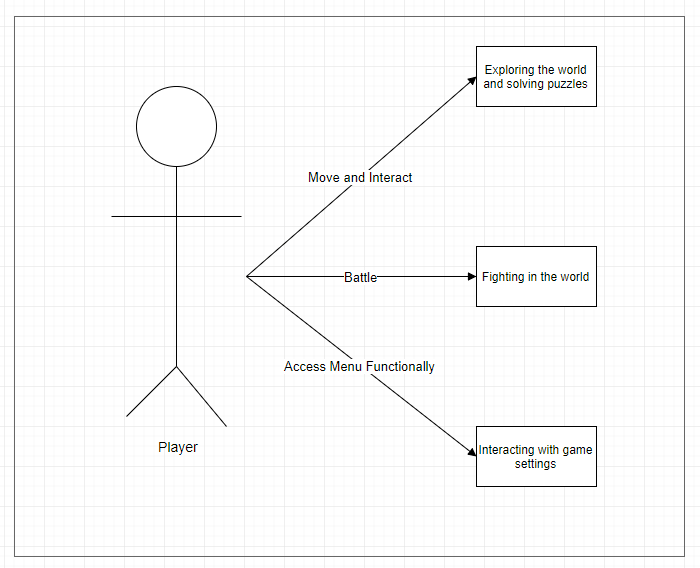
\includegraphics[width=0.8\textwidth]{product-boundary.png} \\
	
	At the current state of the project, the focus will be to complete the fighting mechanic, various character sprite movesets, level design, and Story. Implementing elements of RPG should not be worked on at this time, when the core mechanics are not functional. Features such as combo meter, score system, achievements, and unlockables should be be focused on at later dates if enough development time is available.
	\subsection{Product Use Case (PUC) Table}
	
	\renewcommand{\arraystretch}{2.5}
	\begin{table}[H]
		\begin{tabular}{|l|l|p{4cm}|p{4cm}|
				>{\columncolor[HTML]{C0C0C0}}l lll}
			\hline
			\multicolumn{1}{l|}{\cellcolor[HTML]{C0C0C0}PUC No.}      & \multicolumn{1}{l|}{\cellcolor[HTML]{C0C0C0}PUC Name} & \multicolumn{1}{l|}{\cellcolor[HTML]{C0C0C0}Actor(s)} & \multicolumn{1}{l|}{\cellcolor[HTML]{C0C0C0}Input/Output}                            \\ \hline
			\multicolumn{1}{|l|}{\cellcolor[HTML]{C0C0C0}\textbf{1}}  & \multicolumn{1}{l|}{Moving in game}                   & \multicolumn{1}{l|}{Player}                           & \multicolumn{1}{l|}{Key Input(IN), x-axis position vector(IN/OUT)}                   \\ \hline
			\multicolumn{1}{|l|}{\cellcolor[HTML]{C0C0C0}\textbf{2}}  & \multicolumn{1}{l|}{Jumping in game}                  & \multicolumn{1}{l|}{Player}                           & \multicolumn{1}{l|}{KeyInput(IN), y-axis position vector(IN/OUT)}                    \\ \hline
			\multicolumn{1}{|l|}{\cellcolor[HTML]{C0C0C0}\textbf{3}}  & \multicolumn{1}{l|}{Interacting with items}           & \multicolumn{1}{l|}{Player}                           & \multicolumn{1}{l|}{Key Input(IN), success Boolean(OUT)}                             \\ \hline
			\multicolumn{1}{|l|}{\cellcolor[HTML]{C0C0C0}\textbf{4}}  & \multicolumn{1}{l|}{Viewing Player and Gear Status}   & \multicolumn{1}{l|}{Player}                           & \multicolumn{1}{l|}{Key Input(IN), Player information(OUT)}                          \\ \hline
			\multicolumn{1}{|l|}{\cellcolor[HTML]{C0C0C0}\textbf{5}}  & \multicolumn{1}{l|}{Viewing Items}                    & \multicolumn{1}{l|}{Player}                           & \multicolumn{1}{l|}{Key Input(IN), items menu(OUT)}                                  \\ \hline
			\multicolumn{1}{|l|}{\cellcolor[HTML]{C0C0C0}\textbf{6}}  & \multicolumn{1}{l|}{Performing a melee Attack}        & \multicolumn{1}{l|}{Player}                           & \multicolumn{1}{l|}{Key Input(IN), character sprite Int,(OUT)}                       \\ \hline
			\multicolumn{1}{|l|}{\cellcolor[HTML]{C0C0C0}\textbf{7}}  & \multicolumn{1}{l|}{Performing a ranged Attack}       & \multicolumn{1}{l|}{Player}                           & \multicolumn{1}{l|}{Key Input(IN), character sprite Int,(OUT)}                       \\ \hline
			\multicolumn{1}{|l|}{\cellcolor[HTML]{C0C0C0}\textbf{8}}  & \multicolumn{1}{l|}{Performing a combo Attack}        & \multicolumn{1}{l|}{Player}                           & \multicolumn{1}{l|}{Key Input(IN), character sprite Int,(OUT)}                       \\ \hline
			\multicolumn{1}{|l|}{\cellcolor[HTML]{C0C0C0}\textbf{9}}  & \multicolumn{1}{l|}{Interacting with shop}            & \multicolumn{1}{l|}{Player}                           & \multicolumn{1}{l|}{Key Input(IN), shop menu(OUT)}                                   \\ \hline
			\multicolumn{1}{|l|}{\cellcolor[HTML]{C0C0C0}\textbf{10}} & \multicolumn{1}{l|}{Pausing Game}                     & \multicolumn{1}{l|}{Player}                           & \multicolumn{1}{l|}{Key Input(IN), game menu(OUT)}                                   \\ \hline
			\multicolumn{1}{|l|}{\cellcolor[HTML]{C0C0C0}\textbf{11}} & \multicolumn{1}{l|}{Unpausing game}                   & \multicolumn{1}{l|}{Player}                           & \multicolumn{1}{l|}{Key Input(IN), current game level(OUT)}                          \\ \hline
			\multicolumn{1}{|l|}{\cellcolor[HTML]{C0C0C0}\textbf{12}} & \multicolumn{1}{l|}{Use items}                        & \multicolumn{1}{l|}{Player}                           & \multicolumn{1}{l|}{Key Input(IN), success Boolean(OUT)}                             \\ \hline
			\multicolumn{1}{|l|}{\cellcolor[HTML]{C0C0C0}\textbf{13}} & \multicolumn{1}{l|}{Starting a new game}              & \multicolumn{1}{l|}{Player}                           & \multicolumn{1}{l|}{Key Input(IN), success Boolean(OUT)}                             \\ \hline
			\multicolumn{1}{|l|}{\cellcolor[HTML]{C0C0C0}\textbf{14}} & \multicolumn{1}{l|}{Reaching Checkpoint}              & \multicolumn{1}{l|}{Player}                           & \multicolumn{1}{l|}{Key Input(IN), success Message(OUT)}                             \\ \hline
			\multicolumn{1}{|l|}{\cellcolor[HTML]{C0C0C0}\textbf{15}} & \multicolumn{1}{l|}{Defeating Boss}                   & \multicolumn{1}{l|}{Player}                           & \multicolumn{1}{l|}{Key Input(IN), success Message(OUT)}                             \\ \hline
			\multicolumn{1}{|l|}{\cellcolor[HTML]{C0C0C0}\textbf{16}} & \multicolumn{1}{l|}{Defeating All Enemies}            & \multicolumn{1}{l|}{Player}                           & \multicolumn{1}{l|}{Key Input(IN), success Message(OUT)}                             \\ \hline
			\multicolumn{1}{|l|}{\cellcolor[HTML]{C0C0C0}\textbf{17}} & \multicolumn{1}{l|}{Loading next level}               & \multicolumn{1}{l|}{Player}                           & \multicolumn{1}{l|}{Key Input(IN), success Boolean(OUT)}                             \\ \hline
			\multicolumn{1}{|l|}{\cellcolor[HTML]{C0C0C0}\textbf{18}} & \multicolumn{1}{l|}{Player Death}                     & \multicolumn{1}{l|}{Player}                           & \multicolumn{1}{l|}{health \textless 0 (In), reload checkpoint (OUT)}                \\ \hline
		\end{tabular}
	\end{table}
	
	\begin{table}[H]
		\begin{tabular}{|l|l|p{4cm}|p{4cm}|
				>{\columncolor[HTML]{C0C0C0}}l lll}
			\hline
			\multicolumn{1}{l|}{\cellcolor[HTML]{C0C0C0}PUC No.}      & \multicolumn{1}{l|}{\cellcolor[HTML]{C0C0C0}PUC Name} & \multicolumn{1}{l|}{\cellcolor[HTML]{C0C0C0}Actor(s)} & \multicolumn{1}{l|}{\cellcolor[HTML]{C0C0C0}Input/Output}                            \\ \hline
			\multicolumn{1}{|l|}{\cellcolor[HTML]{C0C0C0}\textbf{19}} & \multicolumn{1}{l|}{Interacting with Gundam Gear}     & \multicolumn{1}{l|}{Player}                           & \multicolumn{1}{l|}{Key Input(IN), success Boolean(OUT)}                             \\ \hline
			\multicolumn{1}{|l|}{\cellcolor[HTML]{C0C0C0}\textbf{20}} & \multicolumn{1}{l|}{View level objectives}            & \multicolumn{1}{l|}{Player}                           & \multicolumn{1}{l|}{Key Input(IN), current Objectives(OUT)}                          \\ \hline
			\multicolumn{1}{|l|}{\cellcolor[HTML]{C0C0C0}\textbf{21}} & \multicolumn{1}{l|}{Entering a new Environment}       & \multicolumn{1}{l|}{Player}                           & \multicolumn{1}{l|}{2d velocity vector(IN), 2d position vector(OUT)}                 \\ \hline
			\multicolumn{1}{|l|}{\cellcolor[HTML]{C0C0C0}\textbf{22}} & \multicolumn{1}{l|}{Viewing achievements}             & \multicolumn{1}{l|}{Player}                           & \multicolumn{1}{l|}{Key Input(IN), Achievement Menu(OUT)}                            \\ \hline
			\multicolumn{1}{|l|}{\cellcolor[HTML]{C0C0C0}\textbf{23}} & \multicolumn{1}{l|}{Exit game}                        & \multicolumn{1}{l|}{Player}                           & \multicolumn{1}{l|}{Key Input(IN)}                                                   \\ \hline
			\multicolumn{1}{|l|}{\cellcolor[HTML]{C0C0C0}\textbf{24}} & \multicolumn{1}{l|}{Selecting new playable character} & \multicolumn{1}{l|}{Player}                           & \multicolumn{1}{l|}{Key Input(IN), success Message(OUT)}                             \\ \hline
			\multicolumn{1}{|l|}{\cellcolor[HTML]{C0C0C0}\textbf{25}} & \multicolumn{1}{l|}{Displaying the Game Settings}     & \multicolumn{1}{l|}{Player}                           & \multicolumn{1}{l|}{Key Input(IN), current game 
				settings(OUT)}                       \\ \hline
			\multicolumn{1}{|l|}{\cellcolor[HTML]{C0C0C0}\textbf{26}} & \multicolumn{1}{l|}{Changing the Game Settings}       & \multicolumn{1}{l|}{Player}                           & \multicolumn{1}{l|}{Key Input(IN), 
				current game settings(OUT)} \\ \hline
			\multicolumn{1}{|l|}{\cellcolor[HTML]{C0C0C0}\textbf{27}} & \multicolumn{1}{l|}{Moving the Camera}                & \multicolumn{1}{l|}{Player}                           & \multicolumn{1}{l|}{2D position vector(IN/OUT)}                                      \\ \hline
			\multicolumn{1}{|l|}{\cellcolor[HTML]{C0C0C0}\textbf{28}} & \multicolumn{1}{l|}{Interacting with Gundam Maintenance}                & \multicolumn{1}{l|}{Player}                           & \multicolumn{1}{l|}{Key Input(IN), Gear upgrading Menu(OUT)}                                      \\ \hline
			
		\end{tabular}
	\end{table}
	
	\newpage
	\subsection{Individual Product Use Cases(PUCs)}
	
	
	\begin{table}[H]
		\begin{tabular}{
				>{\columncolor[HTML]{C0C0C0}}l |p{12cm}|}
			\hline
			\textbf{PUC No.1}& \cellcolor[HTML]{C0C0C0}\textbf{Event: Moving in game}   \\ \hline
			\textbf{Trigger}       & The player presses a key to indicate the direction of the avatar                                                                \\ \hline
			\textbf{Preconditions} & The player is in control of their avatar; Player is in the game world.                                                           \\ \hline
			\textbf{Procedure} & \begin{tabular}[c]{@{}l@{}}1. Add a positive force in the horizontal direction if the right key was pressed. \\Conversely a negative force if the left key was pressed\\ 2. Set the animation to walk \\ 3. If the force is negative flip the direction the character is facing\end{tabular} \\ \hline
			\textbf{Outcome}       & The character moves in a horizontal direction       \\ \hline
		\end{tabular}
	\end{table}
	
	
	
	\begin{table}[H]
		\begin{tabular}{|
				>{\columncolor[HTML]{C0C0C0}}l |p{12cm}|}
			\hline
			\textbf{PUC No.2}      & \cellcolor[HTML]{C0C0C0}\textbf{Event: Jumping in the game}                                                                                                                                                                                                                                     \\ \hline
			\textbf{Trigger}       & The player presses the UP/W on their keyboard                                                                                                                                                                                                                           \\ \hline
			\textbf{Preconditions} & The player is in control of their avatar; Player is in the game world                                                                                                                                                                                                                      \\ \hline
			\textbf{Procedure} & \begin{tabular}[c]{@{}l@{}}1. Move the player’s character upwards along the y-axis for the predetermined
				\\jump height\\ 2.Bring the player’s characters back down, calculating the speed according to\\ gravity, until they collide with a surface.
			\end{tabular} \\ \hline
			\textbf{Outcome}       &The players character moves in a positive direction along the y-axis and comes back down                                                                                                                                                                                                                                              \\ \hline
		\end{tabular}
	\end{table}
	
	
	
	
	\begin{table}[H]
		\begin{tabular}{|
				>{\columncolor[HTML]{C0C0C0}}l |p{12cm}|}
			\hline
			\textbf{PUC No.3}      & \cellcolor[HTML]{C0C0C0}\textbf{Event: Interacting with Items}                                                                                                                                                                                                                                     \\ \hline
			\textbf{Trigger}       & The player presses a key to pick the items                                                                                                                                                                                                                           \\ \hline
			\textbf{Preconditions} & The player is in control of their avatar; Player is in the game world                                                                                                                                                                                                                      \\ \hline
			\textbf{Procedure} & \begin{tabular}[c]{@{}l@{}}
				1. Determine the if the item is within the player’s range\\
				2. Determine the type of the item:\\
				a. If the item is a melee weapon, replace the current melee weapon with the\\ new one, if the current melee weapon is a non - starting weapon, then the old\\ one will drop out.\\
				b. If the item is a ranged weapon, replace the current ranged weapon with the\\ new one, if the old one is a non - starting weapon, then the old one will drop \\out.\\
				c. If the item is a passive item(Power ups), put it in the player’s item bag.\\
				d. If the item is a hp potion, recover player character’s health bar.
				
			\end{tabular} \\ \hline
			\textbf{Outcome}       &The player puts the item in the item bag or recover health bar or get a new weapon         \\ \hline
		\end{tabular}
	\end{table}
	
	
	
	
	\begin{table}[H]
		
		\begin{tabular}{|
				>{\columncolor[HTML]{C0C0C0}}l |p{12cm}|}
			\hline
			\textbf{PUC No.4}      & \cellcolor[HTML]{C0C0C0}\textbf{Event: Viewing Player and Gear Status}                                                                                                                                                                                                                                     \\ \hline
			\textbf{Trigger}       &The player presses the button to open the status menu.                                                                                                                                                                                                                        \\ \hline
			\textbf{Preconditions} & The player is in control of their avatar; Player is in the game world                                                                                                                                                                                                                      \\ \hline
			\textbf{Procedure} & \begin{tabular}[c]{@{}l@{}}
				1.Display the current status of the player and their gear. Clearly labelling all \\information 
				the player needs (current health, ammo count, gundam status etc.)
				
			\end{tabular} \\ \hline
			\textbf{Outcome}       &The players can see the current status of their character and all the gear they have equipped.       \\ \hline
		\end{tabular}
		
	\end{table}
	
	
	\begin{table}[H]
		
		\begin{tabular}{|
				>{\columncolor[HTML]{C0C0C0}}l |p{12cm}|}
			\hline
			\textbf{PUC No.5}      & \cellcolor[HTML]{C0C0C0}\textbf{Event: Viewing Items}                                                                                                                                                                                                                                     \\ \hline
			\textbf{Trigger}       &The player presses i on their keyboard to open up an item’s menu                \\ \hline
			\textbf{Preconditions} & The player must be in the game world                  \\ \hline
			\textbf{Procedure} & \begin{tabular}[c]{@{}l@{}}
				1. Game pauses the current environment and scene \\
				2. An item’s menu is on top of the current environment\\
			\end{tabular} \\ \hline
			\textbf{Outcome}       &An item’s menu appears to a player    \\ \hline
		\end{tabular}
	\end{table}
	
	
	\begin{table}[H]
		\begin{tabular}{|
				>{\columncolor[HTML]{C0C0C0}}l |p{12cm}|}
			\hline
			\textbf{PUC No.6}      & \cellcolor[HTML]{C0C0C0}\textbf{Event: Performing a melee Attack}                                                                                                                                                                                                                                     \\ \hline
			\textbf{Trigger}       &The player presses the button to perform a melee attack              \\ \hline
			\textbf{Preconditions} & The player is in control of their avatar; Player is in the game world                \\ \hline
			\textbf{Procedure} & \begin{tabular}[c]{@{}l@{}}
				1. Determine which type of melee attack the player performed and trigger its \\animation.\\
				2. Determine if the attack is successful by calculating if an enemies hitbox is\\ within range\\ of the attack.\\
				3. Calculate how much HP the enemy will lose\\
				
			\end{tabular} \\ \hline
			\textbf{Outcome}       &The players performs a melee attack on the enemy, resulting them in losing a predetermined amount of HP    \\ \hline
		\end{tabular}
	\end{table}
	
	
	\begin{table}[H]
		\begin{tabular}{|
				>{\columncolor[HTML]{C0C0C0}}l |p{12cm}|}
			\hline
			\textbf{PUC No.7}      & \cellcolor[HTML]{C0C0C0}\textbf{Event: Performing a ranged attack} \\ \hline
			\textbf{Trigger}       &The player presses a button to attack              \\ \hline
			\textbf{Preconditions} & The player is in control of their avatar; Player is in the game world                \\ \hline
			\textbf{Procedure} & \begin{tabular}[c]{@{}l@{}}
				1. Check if any special items are collect that modify the player’s attack\\
				2. Instantiate a projectile prefab (projectile has its own script) in front of the\\ player\\
				3. Add a force to the projectile \\
			\end{tabular} \\ \hline
			\textbf{Outcome}       &The players shoots a projectile   \\ \hline
		\end{tabular}
	\end{table}
	
	\begin{table}[H]
		\begin{tabular}{|
				>{\columncolor[HTML]{C0C0C0}}l |p{12cm}|}
			\hline
			\textbf{PUC No.8}      & \cellcolor[HTML]{C0C0C0}\textbf{Event: Performing a combo Attack} \\ \hline
			\textbf{Trigger}       &The player presses the buttons mapped to a combo attack      \\ \hline
			\textbf{Preconditions} & The player is in control of their avatar; Player is in the game world             \\ \hline
			\textbf{Procedure} & \begin{tabular}[c]{@{}l@{}}
				1. Determine which type of combo attack the player performed and trigger its\\ animation.\\
				2. Determine if the attack is successful by calculating if an enemies hit-box is \\within range of the attack.\\
				3. Calculate how much HP the enemy will lose\\
			\end{tabular} \\ \hline
			\textbf{Outcome}       &The players performs a combo attack on the enemy, resulting them in losing a predetermined amount of HP  \\ \hline
		\end{tabular}
	\end{table}
	
	\begin{table}[H]
		\begin{tabular}{|
				>{\columncolor[HTML]{C0C0C0}}l |p{12cm}|}
			\hline
			\textbf{PUC No.9}      & \cellcolor[HTML]{C0C0C0}\textbf{Event: Interacting with shop} \\ \hline
			\textbf{Trigger}       &The player presses the button to interact with the shop    \\ \hline
			\textbf{Preconditions} & The player is in control of their avatar; Player is in the game world             \\ \hline
			\textbf{Procedure} & \begin{tabular}[c]{@{}l@{}}
				1. Determine if the player is within the range of the shop.\\
				2. A menu list of the shop is on top of the current environment.\\
				3. Calculate how much gold would spend on the selected item.\\
			\end{tabular} \\ \hline
			\textbf{Outcome}       &The player puts the item in the item bag.  \\ \hline
		\end{tabular}
	\end{table}
	
	\begin{table}[H]
		\begin{tabular}{|
				>{\columncolor[HTML]{C0C0C0}}l |p{12cm}|}
			\hline
			\textbf{PUC No.10}      & \cellcolor[HTML]{C0C0C0}\textbf{Event: Pausing the game} \\ \hline
			\textbf{Trigger}       &The player pressing ESC button on keyboard  \\ \hline
			\textbf{Preconditions} & The player is in control of their avatar; Player is in the game world             \\ \hline
			\textbf{Procedure} & \begin{tabular}[c]{@{}l@{}}
				1. Set time scale to zero 
				2. Open a pause menu
			\end{tabular} \\ \hline
			\textbf{Outcome}       &The game is paused  \\ \hline
		\end{tabular}
	\end{table}
	
	
	\begin{table}[H]
		\begin{tabular}{|
				>{\columncolor[HTML]{C0C0C0}}l |p{12cm}|}
			\hline
			\textbf{PUC No.11}      & \cellcolor[HTML]{C0C0C0}\textbf{Event: Unpausing the game} \\ \hline
			\textbf{Trigger}       &The player pressing ESC button on keyboard while game is paused. \\ \hline
			\textbf{Preconditions} & The player is in control of pause menu. Does not control avatar.            \\ \hline
			\textbf{Procedure} & \begin{tabular}[c]{@{}l@{}}
				1. Restore time scale to default\\
				2. Close pause menu\\
				3. Return to game\\
			\end{tabular} \\ \hline
			\textbf{Outcome}       &The game is paused  \\ \hline
		\end{tabular}
	\end{table}
	
	
	\begin{table}[H]
		\begin{tabular}{|
				>{\columncolor[HTML]{C0C0C0}}l |p{12cm}|}
			\hline
			\textbf{PUC No.12}      & \cellcolor[HTML]{C0C0C0}\textbf{Event: Use Items} \\ \hline
			\textbf{Trigger}       &The player press a button mapped to use items \\ \hline
			\textbf{Preconditions} & The player is in control of their avatar; Player is in the game world.         \\ \hline
			\textbf{Procedure} & \begin{tabular}[c]{@{}l@{}}
				1. Player enters item menu \\
				2. Player highlights the item they want to use \\
				3. Player presses to button to use the highlighted items \\
			\end{tabular} \\ \hline
			\textbf{Outcome}       &The player will get hp recovered if they used a potion.  \\ \hline
		\end{tabular}
	\end{table}
	
	\begin{table}[H]
		\begin{tabular}{|
				>{\columncolor[HTML]{C0C0C0}}l |p{12cm}|}
			\hline
			\textbf{PUC No.13}      & \cellcolor[HTML]{C0C0C0}\textbf{Event: Starting a new game} \\ \hline
			\textbf{Trigger}       &The player chooses the “New Game” option from the title screen. \\ \hline
			\textbf{Preconditions} & The player is not currently in an active game session.        \\ \hline
			\textbf{Procedure} & \begin{tabular}[c]{@{}l@{}}
				1. Determine if the start new game button has been selected\\
				2. Display available avatars to choose
				
			\end{tabular} \\ \hline
			\textbf{Outcome}       &The player start the new game and has control of the avatar. \\ \hline
		\end{tabular}
	\end{table}
	
	
	\begin{table}[H]
		\begin{tabular}{|
				>{\columncolor[HTML]{C0C0C0}}l |p{12cm}|}
			\hline
			\textbf{PUC No.14}      & \cellcolor[HTML]{C0C0C0}\textbf{Event: Reaching Checkpoint} \\ \hline
			\textbf{Trigger}       &Having the player avatar collided with an in-game checkpoint, reaching the next level or defeating certain type of enemy\\ \hline
			\textbf{Preconditions} &The player is in control of their avatar; Player is in the game world.      \\ \hline
			\textbf{Procedure} & \begin{tabular}[c]{@{}l@{}}
				1.Determine if the player controls avatar to perform a collision with the\\ checkpoint\\
				2. Set player checkpoint to the most recent checkpoint \\
				
			\end{tabular} \\ \hline
			\textbf{Outcome}       &A message display “Progress has been saved successfully” \\ \hline
		\end{tabular}
	\end{table}
	
	
	
	
	\begin{table}[H]
		\begin{tabular}{|
				>{\columncolor[HTML]{C0C0C0}}l |p{12cm}|}
			\hline
			\textbf{PUC No.15}      & \cellcolor[HTML]{C0C0C0}\textbf{Event: Defeating Boss} \\ \hline
			\textbf{Trigger}       &Boss’s health is reduced to zero\\ \hline
			\textbf{Preconditions} &The player is in control of their character; Located in the game world.     \\ \hline
			\textbf{Procedure} & \begin{tabular}[c]{@{}l@{}}
				1.Determine the chances for boss drops any scrap and gold.
			\end{tabular} \\ \hline
			\textbf{Outcome}       &The player controls avatar to pick up any loot that the Boss was hoarding\\ \hline
		\end{tabular}
	\end{table}
	
	\begin{table}[H]
		\begin{tabular}{|
				>{\columncolor[HTML]{C0C0C0}}l |p{12cm}|}
			\hline
			\textbf{PUC No.16}      & \cellcolor[HTML]{C0C0C0}\textbf{Event: Defeating All Enemies} \\ \hline
			\textbf{Trigger}       &Enemy’s health is reduced to zero\\ \hline
			\textbf{Preconditions} &The player is in control of their character; Located in the game world.    \\ \hline
			\textbf{Procedure} & \begin{tabular}[c]{@{}l@{}}
				1.Determine the chances for enemy drops any scrap. 
			\end{tabular} \\ \hline
			\textbf{Outcome}       &The player controls avatar to pick up any loot that the enemies was hoarding\\ \hline
		\end{tabular}
	\end{table}
	
	\begin{table}[H]
		\begin{tabular}{|
				>{\columncolor[HTML]{C0C0C0}}l |p{12cm}|}
			\hline
			\textbf{PUC No.17}      & \cellcolor[HTML]{C0C0C0}\textbf{Event: Loading next level} \\ \hline
			\textbf{Trigger}       &The player controls avatar reach the destination \\ \hline
			\textbf{Preconditions} &The player is in control of their character; Located in the game world  \\ \hline
			\textbf{Procedure} & \begin{tabular}[c]{@{}l@{}}
				1.Determine and save the inventory and attribute of the player\\
				2.Load the next level and the saved information\\
				
			\end{tabular} \\ \hline
			\textbf{Outcome}       &The player start the new level and has control of the avatar\\ \hline
		\end{tabular}
	\end{table}
	
	
	\begin{table}[H]
		\begin{tabular}{|
				>{\columncolor[HTML]{C0C0C0}}l |p{12cm}|}
			\hline
			\textbf{PUC No.18}      & \cellcolor[HTML]{C0C0C0}\textbf{Event: Player Death } \\ \hline
			\textbf{Trigger}       &The player character’s health is zero\\ \hline
			\textbf{Preconditions} &The player is in control of their character; Located in the game world. \\ \hline
			\textbf{Procedure} & \begin{tabular}[c]{@{}l@{}}
				1. Determine the last saved checkpoint.\\
				2. Restore the player’s avatar to full HP.\\
				
			\end{tabular} \\ \hline
			\textbf{Outcome}       &The player’s avatar is respawned at the last checkpoint.\\ \hline
		\end{tabular}
	\end{table}
	
	\begin{table}[H]
		\begin{tabular}{|
				>{\columncolor[HTML]{C0C0C0}}l |p{12cm}|}
			\hline
			\textbf{PUC No.19}      & \cellcolor[HTML]{C0C0C0}\textbf{Event: Interacting with Gundam Gear } \\ \hline
			\textbf{Trigger}       &Player hits a button mapped to interact with gundum gear  \\ \hline
			\textbf{Preconditions} &The player is in control of their character; Located in the game world.  \\ \hline
			\textbf{Procedure} &
			\begin{tabular}[c]{@{}l@{}}
				1. Determine the if the gear is within the player’s range\\ 
				2. Get in the gear and play gear transformation animation.
				
			\end{tabular} \\ \hline
			\textbf{Outcome}       &The main character is replaced with a new sprite    \\ \hline
		\end{tabular}
	\end{table}
	
	\begin{table}[H]
		\begin{tabular}{|
				>{\columncolor[HTML]{C0C0C0}}l |p{12cm}|}
			\hline
			\textbf{PUC No.20}      & \cellcolor[HTML]{C0C0C0}\textbf{Event: View level objectives} \\ \hline
			\textbf{Trigger}       &  Player hits a button while highlighting in the pause menu  \\ \hline
			\textbf{Preconditions} &    Player must be in the pause menu  associated with the gameworld\\ \hline
			\textbf{Procedure} & \begin{tabular}[c]{@{}l@{}}
				1. Check what the level the player is on\\
				2. Grab the level objective text \\
				3. Show level objective text\\
				
				
			\end{tabular} \\ \hline
			\textbf{Outcome}       &  Objective text is shown to the player  \\ \hline
		\end{tabular}
	\end{table}
	
	
	
	\begin{table}[H]
		\begin{tabular}{|
				>{\columncolor[HTML]{C0C0C0}}l |p{12cm}|}
			\hline
			\textbf{PUC No.21}      & \cellcolor[HTML]{C0C0C0}\textbf{Event: Entering a new Environment } \\ \hline
			\textbf{Trigger}       &Player waits for 5 seconds   \\ \hline
			\textbf{Preconditions} &The player is in control of their character; Located in the game world, all enemies are defeated and boss is cleared    \\ \hline
			\textbf{Procedure} & \begin{tabular}[c]{@{}l@{}}
				1. Kill all enemies and boss or complete puzzle objectives\\
				2. Wait 5 seconds.
				
			\end{tabular} \\ \hline
			\textbf{Outcome}       &Game will load next level.    \\ \hline
		\end{tabular}
	\end{table}
	
	
	\begin{table}[H]
		\begin{tabular}{|
				>{\columncolor[HTML]{C0C0C0}}l |p{12cm}|}
			\hline
			\textbf{PUC No.22}      & \cellcolor[HTML]{C0C0C0}\textbf{Event: Viewing Achievements} \\ \hline
			\textbf{Trigger}       &    The player hits a button while highlighting “View Achievements” in the “Main Menu” \\ \hline
			\textbf{Preconditions} &   The player is in the “Main Menu” \\ \hline
			\textbf{Procedure} & \begin{tabular}[c]{@{}l@{}}
				1. Get achievement list\\
				2. Generate achievement list for print\\
				3. Print achievement list\\
				
				
			\end{tabular} \\ \hline
			\textbf{Outcome}       &   Achievement list  \\ \hline
		\end{tabular}
	\end{table}
	
	
	\begin{table}[H]
		\begin{tabular}{|
				>{\columncolor[HTML]{C0C0C0}}l |p{12cm}|}
			\hline
			\textbf{PUC No.23}      & \cellcolor[HTML]{C0C0C0}\textbf{Event: Exit game  } \\ \hline
			\textbf{Trigger}       &The player hits "ESC" button and select "Return to main menu" or press "alt" + "F4"   \\ \hline
			\textbf{Preconditions} &Player must be in the pause menu  associated with the gameworld    \\ \hline
			\textbf{Procedure} & \begin{tabular}[c]{@{}l@{}}
				1. The player selects "Return to main menu" in the pause menu.
				
			\end{tabular} \\ \hline
			\textbf{Outcome}       &Game exits and main menu shows up    \\ \hline
		\end{tabular}
	\end{table}
	
	
	\begin{table}[H]
		\begin{tabular}{|
				>{\columncolor[HTML]{C0C0C0}}l |p{12cm}|}
			\hline
			\textbf{PUC No.24}      & \cellcolor[HTML]{C0C0C0}\textbf{Event: Selecting new playable character  } \\ \hline
			\textbf{Trigger}       &Player hits button "Enter" while highlighting Playable character  \\ \hline
			\textbf{Preconditions} &Player must be in the character selection menu.    \\ \hline
			\textbf{Procedure} & \begin{tabular}[c]{@{}l@{}}
				1. The player presses "Enter" in the character selection menu.
				
			\end{tabular} \\ \hline
			\textbf{Outcome}       &Player enters the game with the character selected.    \\ \hline
		\end{tabular}
	\end{table}
	
	
	\begin{table}[H]
		\begin{tabular}{|
				>{\columncolor[HTML]{C0C0C0}}l |p{12cm}|}
			\hline
			\textbf{PUC No.25}      & \cellcolor[HTML]{C0C0C0}\textbf{Event: Displaying the Game Settings } \\ \hline
			\textbf{Trigger}       &Player hits "Options" option.   \\ \hline
			\textbf{Preconditions} &Player must be in the main menu/pause menu.    \\ \hline
			\textbf{Procedure} & \begin{tabular}[c]{@{}l@{}}
				1. Player hits "Options" option in main menu/pause menu
				
			\end{tabular} \\ \hline
			\textbf{Outcome}       &The game settings menu shows up    \\ \hline
		\end{tabular}
	\end{table}
	
	
	\begin{table}[H]
		\begin{tabular}{|
				>{\columncolor[HTML]{C0C0C0}}l |p{12cm}|}
			\hline
			\textbf{PUC No.26}      & \cellcolor[HTML]{C0C0C0}\textbf{Event: Changing the Game Settings} \\ \hline
			\textbf{Trigger}       &Player selects the setting options    \\ \hline
			\textbf{Preconditions} &Player must be in the game setting menu    \\ \hline
			\textbf{Procedure} & \begin{tabular}{m{0.80\textwidth}}
				1. Player selects the setting options.\\
				2. a. If the player hits "Apply", then the settings changed will be saved.\\
				\hspace*{0.4cm} b. If the player did not hit apply and player hits "cancel", then the settings change will not be saved.
				
			\end{tabular} \\ \hline
			\textbf{Outcome}       &The game settings are changed/unchanged depends on player's action    \\ \hline
		\end{tabular}
	\end{table}
	
	\begin{table}[H]
		\begin{tabular}{|
				>{\columncolor[HTML]{C0C0C0}}l |p{12cm}|}
			\hline
			\textbf{PUC No.27}      & \cellcolor[HTML]{C0C0C0}\textbf{Event: Moving the Camera} \\ \hline
			\textbf{Trigger}       &Player movement    \\ \hline
			\textbf{Preconditions} &The player is in control of their character; Located in the game world, and the camera is fixed on the player character.     \\ \hline
			\textbf{Procedure} & \begin{tabular}[c]{@{}l@{}}
				1. The player moves, and the camera is fixed on the player character.
				
			\end{tabular} \\ \hline
			\textbf{Outcome}       &The camera moves as player moves    \\ \hline
		\end{tabular}
	\end{table}
	
	
	
	\begin{table}[H]
		\begin{tabular}{|
				>{\columncolor[HTML]{C0C0C0}}l |p{12cm}|}
			\hline
			\textbf{PUC No.28}      & \cellcolor[HTML]{C0C0C0}\textbf{Event: Interacting with Gundam Maintenance} \\ \hline
			\textbf{Trigger}       &The player hits a button mapped to "Interact"    \\ \hline
			\textbf{Preconditions} &The player is in control of their character; Located in the game world    \\ \hline
			\textbf{Procedure} & \begin{tabular}[c]{m{0.80\textwidth}}
				1. Determine if the player is within the range of the Gundam Maintenance.\\
				2. A menu list of the gear is on top of the current environment.\\
				3. Calculate how much scraps would spend on the selected gear for mobile suit upgrade.\\
				4. New mobile suit preview will be present.
				
			\end{tabular} \\ \hline
			\textbf{Outcome}       &The menu of mobile suit upgrade preview will show up    \\ \hline
		\end{tabular}
	\end{table}
	
	
	
	\newpage
	\newpage
	
	
	\section{Functional Requirements}
	\subsection{Core Mechanic}
	\begin{table}[H]
		
		\begin{tabular}{|l|l|l|}
			\hline
			ID:001 & \multicolumn{2}{l|}{Type:Functional Requirement} \\ \hline
			PUC: & \multicolumn{2}{l|}{Originator:Jonathan Yu} \\ \hline
			Description & \multicolumn{2}{m{0.85\textwidth}|}{When the player’s avatar enters a level, a fixed amount of enemies are created. If all enemies are destroyed than, the game will load,to the next level.} \\ \hline
			Rationale & \multicolumn{2}{m{0.85\textwidth}|}{To prevent the player from accessing a part of the level and creating a natural boundary for the intended game world. A fail condition for the player} \\ \hline
			Fit Criterion & \multicolumn{2}{m{0.85\textwidth}|}{\begin{tabular}[c]{@{}l@{}}1. Fixed number of enemies will be spawned when level is loaded. Enemy will spawn at fixed locations. Enemies aggro when player is within range.\\ 2. When enemy counter reaches zero, level completes.\end{tabular}} \\ \hline
			Satisfaction: 5 & Dissatisfaction: 5 & Priority: Very High \\ \hline
			Conflicts:N/A & \multicolumn{2}{l|}{Supporting Material:N/A} \\ \hline
		\end{tabular}
		
	\end{table}
	
	\begin{table}[H]
		
		\begin{tabular}{|l|l|l|}
			\hline
			ID:002 & \multicolumn{2}{l|}{Type:Functional Requirement} \\ \hline
			PUC: & \multicolumn{2}{l|}{Originator:Jonathan Yu} \\ \hline
			Description & \multicolumn{2}{m{0.85\textwidth}|}{When the player’s collides with an invisible preset boundary, the game reloads the level and the player’s lives are decremented by one, if the the players lives are less than 0 then the game loads the game over scene.} \\ \hline
			Rationale & \multicolumn{2}{m{0.85\textwidth}|}{To prevent the player from accessing a part of the level and creating a natural boundary for the intended game world. A fail condition for the player} \\ \hline
			Fit Criterion & \multicolumn{2}{m{0.85\textwidth}|}{Assert if the instance of the object and the player that collided with each other are still within the scene} \\ \hline
			Satisfaction: 5 & Dissatisfaction: 5 & Priority: Very High \\ \hline
			Conflicts:N/A & Supporting Material:N/A &  \\ \hline
		\end{tabular}
	\end{table}
	
	
	
	\begin{table}[H]
		\begin{tabular}{|l|l|l|}
			\hline
			ID:003 & \multicolumn{2}{l|}{Type:Functional Requirement} \\ \hline
			PUC: 18 & \multicolumn{2}{l|}{Originator:Jonathan Yu} \\ \hline
			Description & \multicolumn{2}{m{0.85\textwidth}|}{When the player’s collides with an enemy, the player loses a percentage of their total health depending on what enemy he collided with, if the player’s health reaches below zero than the game reloads the current level and the player’s lives are decremented by one, if the the players lives are less than 0 then the game loads the game over scene.} \\ \hline
			Rationale & \multicolumn{2}{m{0.85\textwidth}|}{One of the primary fail conditions for the player} \\ \hline
			Fit Criterion & \multicolumn{2}{m{0.85\textwidth}|}{Assert if the instance of the object and the player that collided with each other are still within the scene} \\ \hline
			Satisfaction: 4 & Dissatisfaction: 5 & Priority: Very High \\ \hline
			Conflicts:N/A & \multicolumn{2}{l|}{Supporting Material:N/A} \\ \hline
		\end{tabular}
	\end{table}
	
	
	\begin{table}[H]
		\begin{tabular}{|l|l|l|}
			\hline
			ID:004 & \multicolumn{2}{l|}{Type:Functional Requirement} \\ \hline
			PUC: 2& \multicolumn{2}{l|}{Originator:Jonathan Yu} \\ \hline
			Description & \multicolumn{2}{m{0.85\textwidth}|}{All characters in the game screen will be subjected to gravity, a downward force in the negative Y direction every ms.} \\ \hline
			Rationale & \multicolumn{2}{m{0.85\textwidth}|}{Define one constant rate of downward motion.} \\ \hline
			Fit Criterion & \multicolumn{2}{m{0.85\textwidth}|}{Use Rigid Body property of Unity} \\ \hline
			Satisfaction: 5 & Dissatisfaction: 5 & Priority: Very High \\ \hline
			Conflicts:N/A & \multicolumn{2}{l|}{Supporting Material:N/A} \\ \hline
		\end{tabular}
	\end{table}
	
	\begin{table}[H]
		\begin{tabular}{|l|l|l|}
			\hline
			ID:005 & \multicolumn{2}{l|}{Type:Functional Requirement} \\ \hline
			PUC: 18& \multicolumn{2}{l|}{Originator:Jonathan Yu} \\ \hline
			Description & \multicolumn{2}{m{0.85\textwidth}|}{Al characters will have their own health pool.}\\\hline
			Rationale & \multicolumn{2}{m{0.85\textwidth}|}{Mobiles suits can only sustain so much damage before they are destroyed, health points are used as a representation of the about of damage  they can take. For game play experience and real life representation, different machines will have various amounts of hp. Boss characters will have the most.} \\ \hline
			Fit Criterion & \multicolumn{2}{m{0.85\textwidth}|}{Set various HP amount for characters.} \\ \hline
			Satisfaction: 5 & Dissatisfaction: 5 & Priority: Very High \\ \hline
			Conflicts:N/A & \multicolumn{2}{l|}{Supporting Material:N/A} \\ \hline
		\end{tabular}
	\end{table}
	
	
	\begin{table}[H]
		\begin{tabular}{|l|l|l|}
			\hline
			ID:006& \multicolumn{2}{l|}{Type:Functional Requirement} \\ \hline
			PUC: 18& \multicolumn{2}{l|}{Originator:Jonathan Yu} \\ \hline
			Description & \multicolumn{2}{m{0.85\textwidth}|}{When the player attacks, he will instantiate a new box collider that covers the range of his attack, if that box collides with another object it loses a percentage  of their health that is scaled by the player’s attack, if their health goes below zero than play the death animation and destroy the object.}\\\hline
			Rationale & \multicolumn{2}{m{0.85\textwidth}|}{The rides in a mobile suit as a weapon the player needs a means to destroy the enemy mobile suits} \\ \hline
			Fit Criterion & \multicolumn{2}{m{0.85\textwidth}|}{New box collider for select animation frames. On collision with enemy box, decrease enemy health.} \\ \hline
			Satisfaction: 5 & Dissatisfaction: 5 & Priority: Very High \\ \hline
			Conflicts:N/A & \multicolumn{2}{l|}{Supporting Material:N/A} \\ \hline
		\end{tabular}
	\end{table}
	
	
	\begin{table}[H]
		\begin{tabular}{|l|l|l|}
			\hline
			ID:007&\multicolumn{2}{l|}{Type:Functional Requirement} \\ \hline
			PUC: 1& \multicolumn{2}{l|}{Originator:Jonathan Yu} \\ \hline
			Description & \multicolumn{2}{m{0.85\textwidth}|}{The player’s avatar should be able to move on the horizontal axis }\\\hline
			Rationale & \multicolumn{2}{m{0.85\textwidth}|}{Avatar should be able to explore the level with the ability to move horizontally.} \\ \hline
			Fit Criterion & \multicolumn{2}{m{0.85\textwidth}|}{Avatar move towards left when “Left” key is pressed. Avatar move towards right when “Right” key is pressed.} \\ \hline
			Satisfaction: 4 & Dissatisfaction: 5 & Priority: Very High \\ \hline
			Conflicts:N/A & \multicolumn{2}{l|}{Supporting Material:N/A} \\ \hline
		\end{tabular}
	\end{table}
	
	
	\begin{table}[H]
		\begin{tabular}{|l|l|l|}
			\hline
			ID:008&\multicolumn{2}{l|}{Type:Functional Requirement} \\ \hline
			PUC: 2& \multicolumn{2}{l|}{Originator:Jonathan Yu} \\ \hline
			Description & \multicolumn{2}{m{0.85\textwidth}|}{The player’s avatar should be able to jump, achieved by adding a vertical force in the positive Y direction }\\\hline
			Rationale & \multicolumn{2}{m{0.85\textwidth}|}{.Avatar should be able to explore the level with the ability to move Vertically.} \\ \hline
			Fit Criterion & \multicolumn{2}{m{0.85\textwidth}|}{Avatar gain positive Y velocity when  “Space” key is pressed. Velocity decreases overtime due to gravity.} \\ \hline
			Satisfaction: 4 & Dissatisfaction: 5 & Priority: Very High \\ \hline
			Conflicts:N/A & \multicolumn{2}{l|}{Supporting Material:N/A} \\ \hline
		\end{tabular}
	\end{table}
	
	\begin{table}[H]
		\begin{tabular}{|l|l|l|}
			\hline
			ID:009 & \multicolumn{2}{l|}{Type:Functional Requirement} \\ \hline
			PUC:3 & \multicolumn{2}{l|}{Originator:Jonathan Yu} \\ \hline
			Description & \multicolumn{2}{m{0.85\textwidth}|}{Ensure that the attributes that have been modified are accurate,with a formula} \\ \hline
			Rationale & \multicolumn{2}{m{0.85\textwidth}|}{It gives the player a feel of progression, making his machine stronger the longer he plays, and gives him a sub goal. The idea is about destroying your enemies and taking their gear to bolster your own} \\ \hline
			Fit Criterion & \multicolumn{2}{m{0.85\textwidth}|}{ \begin{tabular}{m{0.8\textwidth}}When the player collides with an item his attributes are changed depending on the type of item. For example if he collects and attack upgrade, he will do a larger \% of damage.\\ 1. There will be damage upgrade items. When Avatar collides with item, there will be a multiplier to attack value.\\ 2. There will be speed upgrade items. When Avatar collides with item, there will be multiplier to movement speed and jump velocity value.\\ 3. There will be health upgrade items. When Avatar collides with item, maximum health value will be increased.\\ 4. There will be usable items. When Avatar collides with item, item will be added to inventory, can be used by pressing the designated button and item will no longer be in inventory.\end{tabular}} \\ \hline
			Satisfaction: 5 & Dissatisfaction: 5 & Priority: Medium \\ \hline
			Conflicts:N/A & \multicolumn{2}{l|}{Supporting Material:N/A} \\ \hline
		\end{tabular}
	\end{table}
	
	\subsection{Primary Gameplay Mode}
	
	
	\begin{table}[H]
		\begin{tabular}{|l|l|l|}
			\hline
			ID:010 & \multicolumn{2}{l|}{Type:Functional Requirement} \\ \hline
			PUC: 21 & \multicolumn{2}{l|}{Originator:} \\ \hline
			Description & \multicolumn{2}{m{0.85\textwidth}|}{The primary gameplay mode will be Story Mission Mode where players shall complete the each levels of the game. The win condition is to complete all levels.} \\ \hline
			Rationale & \multicolumn{2}{m{0.85\textwidth}|}{Primary mode should be able to explore all levels by sequence and present the story.} \\ \hline
			Fit Criterion & \multicolumn{2}{m{0.85\textwidth}|}{} \\ \hline
			Satisfaction: & Dissatisfaction: & Priority: Very High\\ \hline
			Conflicts: & \multicolumn{2}{l|}{Supporting Material:} \\ \hline
		\end{tabular}
	\end{table}
	
	\subsection{Alternate Game Modes}
	
	
	\begin{table}[H]
		\begin{tabular}{|l|l|l|}
			\hline
			ID:011 & \multicolumn{2}{l|}{Type:Functional Requirement} \\ \hline
			PUC: 24, 26 & \multicolumn{2}{l|}{Originator:} \\ \hline
			Description & \multicolumn{2}{m{0.85\textwidth}|}{Free Mission Mode allows player can choose which playable character to use and which level to play. After select level is completed, return to mission select screen.} \\ \hline
			Rationale & \multicolumn{2}{m{0.85\textwidth}|}{Alternate mode grants player more freedom. } \\ \hline
			Fit Criterion & \multicolumn{2}{m{0.85\textwidth}|}{} \\ \hline
			Satisfaction: & Dissatisfaction: & Priority: Medium\\ \hline
			Conflicts: & \multicolumn{2}{l|}{Supporting Material:} \\ \hline
		\end{tabular}
	\end{table}
	
	\begin{table}[H]
		\begin{tabular}{|l|l|l|}
			\hline
			ID:012 & \multicolumn{2}{l|}{Type:Functional Requirement} \\ \hline
			PUC: 25, 26 & \multicolumn{2}{l|}{Originator: Tian Guo} \\ \hline
			Description & \multicolumn{2}{m{0.85\textwidth}|}{A start menu that allows the player to select Story Mission Mode, Free Mission Mode, Options to change game settings, and Exit to terminate the game.} \\ \hline
			Rationale & \multicolumn{2}{m{0.85\textwidth}|}{Game should begin at menu to give player option to choose how to play and options to change settings.} \\ \hline
			Fit Criterion & \multicolumn{2}{m{0.85\textwidth}|}{\begin{tabular}[c]{@{}l@{}}1. Game will boot into start menu.\\ 2. Start menu shall contain Story Mission, Free Mission, Option, and Exit buttons.\\ 3. Each button will execute the relevant functions.\end{tabular}} \\ \hline
			Satisfaction: & Dissatisfaction: & Priority: Very High\\ \hline
			Conflicts: & \multicolumn{2}{l|}{Supporting Material:} \\ \hline
		\end{tabular}
	\end{table}
	
	\begin{table}[H]
		\begin{tabular}{|l|l|l|}
			\hline
			ID:013 & \multicolumn{2}{l|}{Type:Functional Requirement} \\ \hline
			PUC:10, 11, 25, 26 & \multicolumn{2}{l|}{Originator: Tian Guo} \\ \hline
			Description & \multicolumn{2}{m{0.85\textwidth}|}{During game missions the player can open the pause menu to pause the game. The menu will consist of “Resume” to unpause the game from pause menu, Options to change certain settings, and Back to Title to return to main menu.} \\ \hline
			Rationale & \multicolumn{2}{m{0.85\textwidth}|}{During missions, player should have the ability to open pause menu if need be. Play can change settings in this screen if adjustments are needed.} \\ \hline
			Fit Criterion & \multicolumn{2}{m{0.85\textwidth}|}{\begin{tabular}[c]{@{}l@{}}1.During mission player shall be able to open pause menu by pressing “ESC” key.\\ 2. Pause menu shall pause the game until the menu is closed.\\ 3. Pause menu shall have resume, options, and back to title buttons.\\ 4. Pressing “ESC” again while in pause menu shall resume the game as well.\end{tabular}} \\ \hline
			Satisfaction: & Dissatisfaction: & Priority: High\\ \hline
			Conflicts: & \multicolumn{2}{l|}{Supporting Material:} \\ \hline
		\end{tabular}
	\end{table}
	
	\section{Look and Feel Requirements}
	\subsection{Appearance Requirements}
	\begin{table}[H]
		\begin{tabular}{|l|l|l|}
			\hline
			ID:101 & \multicolumn{2}{l|}{Non-Functional Requirement(Appearance)} \\ \hline
			PUC: 1, 2, 10, 25, 26 & \multicolumn{2}{l|}{Originator: Tian Guo} \\ \hline
			Description & \multicolumn{2}{m{0.85\textwidth}|}{Characters must look distinct from each other. Player must be able to tell difference between the player avatar and enemy easily. Foreground and background must differentiate easily.} \\ \hline
			Rationale & \multicolumn{2}{m{0.85\textwidth}|}{Object on screen must represent itself clearly} \\ \hline
			Fit Criterion & \multicolumn{2}{m{0.85\textwidth}|}{\begin{tabular}[c]{@{}l@{}}1.Player can easily distinguish self from others.\\ 2. Player can easily distinguish foreground and background\end{tabular}} \\ \hline
			Satisfaction: & Dissatisfaction: & Priority: High\\ \hline
			Conflicts: & \multicolumn{2}{l|}{Supporting Material:} \\ \hline
		\end{tabular}
	\end{table}
	
	\subsection{Style Requirements}
	
	\begin{table}[H]
		\begin{tabular}{|l|l|l|}
			\hline
			ID:101 & \multicolumn{2}{l|}{Type:Non-Functional Requirement(Look and Feel - Style)} \\ \hline
			PUC: 19, 21 & \multicolumn{2}{m{0.85\textwidth}|}{Originator: Tian Guo} \\ \hline
			Description & \multicolumn{2}{m{0.85\textwidth}|}{Objects in the game must exert futuristic style} \\ \hline
			Rationale & \multicolumn{2}{m{0.85\textwidth}|}{The look of the game should reflect the Sci-Fi setting} \\ \hline
			Fit Criterion & \multicolumn{2}{m{0.85\textwidth}|}{Objects should look mechanical, has electronics, or seems to be made from metal.} \\ \hline
			Satisfaction: & Dissatisfaction: & Priority: High\\ \hline
			Conflicts: & \multicolumn{2}{l|}{Supporting Material:} \\ \hline
		\end{tabular}
	\end{table}
	
	\begin{table}[H]
		\begin{tabular}{|l|l|l|}
			\hline
			ID:102 & \multicolumn{2}{l|}{Type:Non-Functional Requirement(Look and Feel - Style)} \\ \hline
			PUC: 2, 6, 7, 8 & \multicolumn{2}{l|}{Originator: Tian Guo} \\ \hline
			Description & \multicolumn{2}{m{0.85\textwidth}|}{Playing the game must feel like mix of action and platforming} \\ \hline
			Rationale & \multicolumn{2}{m{0.85\textwidth}|}{Playing the game should feel like brawler or fighting game from the combat mechanic. Traversing the game should feel like platformer and Metroidvania games.} \\ \hline
			Fit Criterion & \multicolumn{2}{m{0.85\textwidth}|}{Game should have solid fighting game mechanics and platformer level design.} \\ \hline
			Satisfaction: & Dissatisfaction: & Priority: High\\ \hline
			Conflicts: & \multicolumn{2}{l|}{Supporting Material:} \\ \hline
		\end{tabular}
	\end{table}
	
	\subsection{Requisite Assets}
	\subsubsection{Audio}
	\begin{table}[H]
		\begin{tabular}{|1|1|1|}
			\hline
			Asset Type & Number Required & Rationale\\ \hline
			Character Sound Effect & 2  &\multicolumn{1}{m{0.45\textwidth}|}{Require minimum two sets for playable characters' sound effects} \\ \hline
			Enemy Character Sound Effects & 6  &\multicolumn{1}{m{0.45\textwidth}|}{Require minimum 6 different sets of sound effects for enemy types and bosses}\\ \hline
			Background Sound Track & 6  &\multicolumn{1}{m{0.45\textwidth}|}{Require minimum 6 Tracks for different scenery} \\ \hline
		\end{tabular}
	\end{table}
	\subsubsection{Visual}
	\begin{table}[H]
		\begin{tabular}{|1|1|1|}
			\hline
			Asset Type & Number Required & Rationale\\ \hline
			Main Character Sprite & 2 Sets &\multicolumn{1}{m{0.5\textwidth}|}{Require minimum two sets for playable } \\ \hline
			Enemy Character Sprite & 6 Sets &\multicolumn{1}{m{0.5\textwidth}|}{ Require minimum 6 different enemy types and bosses}\\ \hline
			Background Sprite & 6 Sets &\multicolumn{1}{m{0.5\textwidth}|}{ Require minimum 6 sets for different scenery}\\ \hline
			Foreground Sprite & 6 Sets &\multicolumn{1}{m{0.5\textwidth}|}{ Require minimum 6 sets for foreground objects and platforms}\\ \hline
		\end{tabular}
	\end{table}
	
	
	\section{Usability and Humanity Requirements}
	\subsection{Ease of Use Requirements}
	\begin{table}[H]
		\begin{tabular}{|l|l|l|}
			\hline
			ID:201 & \multicolumn{2}{l|}{Type: Non-Functional Requirement(Ease of Use)} \\ \hline
			PUC: 1, 2, 20 & \multicolumn{2}{l|}{Originator: Tian Guo} \\ \hline
			Description & \multicolumn{2}{m{0.85\textwidth}|}{Requirement on how easily player can play the game physically.} \\ \hline
			Rationale & \multicolumn{2}{m{0.85\textwidth}|}{Player should not be hindered by the controls while playing} \\ \hline
			Fit Criterion & \multicolumn{2}{m{0.85\textwidth}|}{Button layout for controlling player avatar must be intuitive and similar to other games of the genre.} \\ \hline
			Satisfaction: 5 & Dissatisfaction: 5 & Priority: Very High \\ \hline
			Conflicts: N/A & \multicolumn{2}{l|}{Supporting Material: N/A} \\ \hline
		\end{tabular}
	\end{table}
	
	\subsection{Personalization Requirements}
	\begin{table}[H]
		\begin{tabular}{|l|l|l|}
			\hline
			ID:202 & \multicolumn{2}{l|}{Type: Non-Functional Requirement(Personalization)} \\ \hline
			PUC: 26 & \multicolumn{2}{l|}{Originator: Saim Zahid} \\ \hline
			Description & \multicolumn{2}{m{0.85\textwidth}|}{Customization requirements} \\ \hline
			Rationale & \multicolumn{2}{m{0.85\textwidth}|}{Player should be able to play the game as per personal preference.} \\ \hline
			Fit Criterion & \multicolumn{2}{m{0.85\textwidth}|}{Player must be able to change the video and audio settings, pausing and unpausing the game, and changing the mobile suit of the character as per preference.} \\ \hline
			Satisfaction: 5 & Dissatisfaction: 5 & Priority: Very High \\ \hline
			Conflicts: N/A & \multicolumn{2}{l|}{Supporting Material: N/A} \\ \hline
		\end{tabular}
	\end{table}
	
	
	\subsection{Learning Requirements}
	\begin{table}[H]
		\begin{tabular}{|l|l|l|}
			\hline
			ID:203 & \multicolumn{2}{l|}{Type:Non-Functional Requirement(Learning)} \\ \hline
			PUC: & \multicolumn{2}{l|}{Originator: Tian Guo} \\ \hline
			Description & \multicolumn{2}{m{0.85\textwidth}|}{Requirement of how easily a new player should be able to pick up the game} \\ \hline
			Rationale & \multicolumn{2}{m{0.85\textwidth}|}{Player should not spend large amount of time to learn to play the game} \\ \hline
			Fit Criterion & \multicolumn{2}{m{0.85\textwidth}|}{The main control and concept of the game must be very intuitive and easy to learn. Player must be able to grasp the control of the game within few minutes of first stage.} \\ \hline
			Satisfaction: 5 & Dissatisfaction: 5 & Priority: Very High \\ \hline
			Conflicts: N/A & \multicolumn{2}{l|}{Supporting Material: N/A} \\ \hline
		\end{tabular}
	\end{table}
	
	\subsection{Understandability and Politeness Requirements}
	\begin{table}[H]
		\begin{tabular}{|l|l|l|}
			\hline
			ID:204 & \multicolumn{2}{l|}{Type:Non-Functional Requirement(Understandability and Politeness)} \\ \hline
			PUC:1, 2, 6, 7, 8, 14, 15, 16 & \multicolumn{2}{l|}{Originator: Yicheng Chen} \\ \hline
			Description & \multicolumn{2}{m{0.85\textwidth}|}{Requirement of how easily a player understand the game and in what level of politeness that the language of the game is representing.} \\ \hline
			Rationale & \multicolumn{2}{m{0.85\textwidth}|}{Players should not have a hard time understanding the language of the game. The dialogue and context should not contain hate speech} \\ \hline
			Fit Criterion & \multicolumn{2}{m{0.85\textwidth}|}{The conversation, subtitles, naming, lores must be in English and have appropriate grammar. And they should not contain hate speech at all. Players must have a comfortable gaming environment during the game.} \\ \hline
			Satisfaction: 5 & Dissatisfaction: 5 & Priority: Very High \\ \hline
			Conflicts: N/A & \multicolumn{2}{l|}{Supporting Material: N/A} \\ \hline
		\end{tabular}
	\end{table}
	
	\subsection{Accessibility Requirements}
	\begin{table}[H]
		\begin{tabular}{|l|l|l|}
			\hline
			ID:205 & \multicolumn{2}{l|}{Type:Non-Functional Requirement(Accessibility)} \\ \hline
			PUC: 1 & \multicolumn{2}{l|}{Originator: Tian Guo} \\ \hline
			Description & \multicolumn{2}{m{0.85\textwidth}|}{How easily targeted audience can get ahold of the product} \\ \hline
			Rationale & \multicolumn{2}{m{0.85\textwidth}|}{Game should be playable on common hardware and platforms.} \\ \hline
			Fit Criterion & \multicolumn{2}{m{0.85\textwidth}|}{The program must be able to run on PC, Mac, and Linux platforms.} \\ \hline
			Satisfaction: 5 & Dissatisfaction: 5 & Priority: Very High \\ \hline
			Conflicts: N/A & \multicolumn{2}{l|}{Supporting Material: N/A} \\ \hline
		\end{tabular}
	\end{table}
	
	\section{Performance Requirements}
	\subsection{Speed and Latency Requirements}
	\begin{table}[H]
		\begin{tabular}{|l|l|l|}
			\hline
			ID:206 & \multicolumn{2}{l|}{Type:Non-Functional Requirement(Performance - Speed and Latency)} \\ \hline
			PUC: 1, 2, 6, 7, 8  & \multicolumn{2}{l|}{Originator: Tian Guo} \\ \hline
			Description & \multicolumn{2}{m{0.85\textwidth}|}{Requirement of how fast and responsive the game should be.} \\ \hline
			Rationale & \multicolumn{2}{m{0.85\textwidth}|}{Due to the game’s genre as a platformer and the focus on combos, the game must feel very responsive. The game’s theme is Sci-Fi and Mecha, therefore the speed does not need to be very fast.} \\ \hline
			Fit Criterion & \multicolumn{2}{m{0.85\textwidth}|}{Players input must not have large latency. The latency should be below 90ms and unnoticeable to the player.} \\ \hline
			Satisfaction: 5 & Dissatisfaction: 5 & Priority: Very High \\ \hline
			Conflicts: N/A & \multicolumn{2}{l|}{Supporting Material: N/A} \\ \hline
		\end{tabular}
	\end{table}
	
	\subsection{Precision or Accuracy Requirements}
	\begin{table}[H]
		\begin{tabular}{|l|l|l|}
			\hline
			ID:207 & \multicolumn{2}{l|}{Type:Non-Functional Requirement(Performance - Precision or Accuracy)} \\ \hline
			PUC: 6, 7, 8 & \multicolumn{2}{l|}{Originator: Tian Guo} \\ \hline
			Description & \multicolumn{2}{m{0.85\textwidth}|}{Requirement of how accurate and precise hitboxes are.} \\ \hline
			Rationale & \multicolumn{2}{m{0.85\textwidth}|}{Unlike traditional fighting games, there will not be high, mid, and low strikes and blocks. The hitbox of characters will be more lenient than games such as Tekken, Street Fighter, or Mortal Kombat.} \\ \hline
			Fit Criterion & \multicolumn{2}{m{0.85\textwidth}|}{If the attack appears to have landed on enemies, the hit must register.} \\ \hline
			Satisfaction: 5 & Dissatisfaction: 5 & Priority: Very High \\ \hline
			Conflicts: N/A & \multicolumn{2}{l|}{Supporting Material: N/A} \\ \hline
		\end{tabular}
	\end{table}
	
	\subsection{Reliability and Availability Requirements}
	\begin{table}[H]
		\begin{tabular}{|l|l|l|}
			\hline
			ID:208 & \multicolumn{2}{l|}{Type:Non-Functional Requirement(Performance - Reliability and Availability)} \\ \hline
			PUC: All & \multicolumn{2}{l|}{Originator: Yicheng Chen} \\ \hline
			Description & \multicolumn{2}{m{0.85\textwidth}|}{Requirement for party of liability and availability of the party.} \\ \hline
			Rationale & \multicolumn{2}{m{0.85\textwidth}|}{Game should have reliable party. And game should have available support.} \\ \hline
			Fit Criterion & \multicolumn{2}{m{0.85\textwidth}|}{Development team must be liable for all issues of the game. Dev team must be available to solve issues before April 28th 2018.} \\ \hline
			Satisfaction: 5 & Dissatisfaction: 5 & Priority: Very High \\ \hline
			Conflicts: N/A & \multicolumn{2}{l|}{Supporting Material: N/A} \\ \hline
		\end{tabular}
	\end{table}
	
	\subsection{Robustness or Fault Tolerance Requirements}
	\begin{table}[H]
		\begin{tabular}{|l|l|l|}
			\hline
			ID:209 & \multicolumn{2}{l|}{Type:Non-Functional Requirement(Performance - Robustness or Fault Tolerance)} \\ \hline
			PUC: All & \multicolumn{2}{l|}{Originator: Tian Guo} \\ \hline
			Description & \multicolumn{2}{m{0.85\textwidth}|}{Requirement of the frequency of crashes and unexpected errors.} \\ \hline
			Rationale & \multicolumn{2}{m{0.85\textwidth}|}{Any crashes or unexpected errors that disrupts gameplay should not be occuring.} \\ \hline
			Fit Criterion & \multicolumn{2}{m{0.85\textwidth}|}{The game will not crash unexpectedly under normal circumstances. The game will perform at acceptable level on all platform and machines that it is running on.} \\ \hline
			Satisfaction: 5 & Dissatisfaction: 5 & Priority: Very High \\ \hline
			Conflicts: N/A & \multicolumn{2}{l|}{Supporting Material: N/A} \\ \hline
		\end{tabular}
	\end{table}
	
	\subsection{Capacity Requirements}
	\begin{table}[H]
		\begin{tabular}{|l|l|l|}
			\hline
			ID:210 & \multicolumn{2}{l|}{Type:Non-Functional Requirement(Performance - Capacity)} \\ \hline
			PUC:1, 17, 21 & \multicolumn{2}{l|}{Originator: Yichneg Chen} \\ \hline
			Description & \multicolumn{2}{m{0.85\textwidth}|}{The system should be able to create and maintain at most thirty(30) characters in one game level, and at most ten(10) characters on the screen.} \\ \hline
			Rationale & \multicolumn{2}{m{0.85\textwidth}|}{With too many characters showing up on one screen could dramtically affect game performance.} \\ \hline
			Fit Criterion & \multicolumn{2}{m{0.85\textwidth}|}{The game must allow thirty characters to show up in one level, ten characters show up while system performance is not affected too much.} \\ \hline
			Satisfaction: 5 & Dissatisfaction: 5 & Priority: Very High \\ \hline
			Conflicts: N/A & \multicolumn{2}{l|}{Supporting Material: N/A} \\ \hline
		\end{tabular}
	\end{table}
	
	\section{Scalability and Extensibility Requirements}
	\begin{table}[H]
		\begin{tabular}{|l|l|l|}
			\hline
			ID:211 & \multicolumn{2}{l|}{Type:Scalability} \\ \hline
			PUC: All & \multicolumn{2}{l|}{Originator: Yichneg Chen} \\ \hline
			Description & \multicolumn{2}{m{0.85\textwidth}|}{The game should be coded in a way where adding new levels are possible without changing previously written code} \\ \hline
			Rationale & \multicolumn{2}{m{0.85\textwidth}|}{The game can be expanded upon later, downloadable content could be added, most importantly code can be reused for different games.} \\ \hline
			Fit Criterion & \multicolumn{2}{m{0.85\textwidth}|}{The player must be able to play the game for at least fifteen minutes, and the player must be able to explore} \\ \hline
			Satisfaction: 5 & Dissatisfaction: 5 & Priority: Very High \\ \hline
			Conflicts: N/A & \multicolumn{2}{l|}{Supporting Material: N/A} \\ \hline
		\end{tabular}
	\end{table}
	
	\section{Longevity Requirements}
	\begin{table}[H]
		\begin{tabular}{|l|l|l|}
			\hline
			ID:212 & \multicolumn{2}{l|}{Type:Non-Functional Requirement(Performance - Longevity)} \\ \hline
			PUC: All & \multicolumn{2}{l|}{Originator: Yichneg Chen} \\ \hline
			Description & \multicolumn{2}{m{0.85\textwidth}|}{Requirement of a minimum of Fifteen(15) minutes game play to be played by the players.} \\ \hline
			Rationale & \multicolumn{2}{m{0.85\textwidth}|}{The final product should be able to be played for a minimum of fifteen(15) minutes for graded demonstration.} \\ \hline
			Fit Criterion & \multicolumn{2}{m{0.85\textwidth}|}{The player must be able to play the game for at least fifteen minutes. And the player must be able to explore} \\ \hline
			Satisfaction: 5 & Dissatisfaction: 5 & Priority: Very High \\ \hline
			Conflicts: N/A & \multicolumn{2}{l|}{Supporting Material: N/A} \\ \hline
		\end{tabular}
	\end{table}
	
	\section{Operational and Environmental Requirements}
	\begin{table}[H]
		\begin{tabular}{|l|l|l|}
			\hline
			ID:213 & \multicolumn{2}{l|}{Type:Operational and Environmental Requirements} \\ \hline
			PUC: All & \multicolumn{2}{l|}{Originator: Jonathan Yu} \\ \hline
			Description & \multicolumn{2}{m{0.85\textwidth}|}{The game will not overuse the CPU or overheat the power supply} \\ \hline
			Rationale & \multicolumn{2}{m{0.85\textwidth}|}{This could cause an explosion potentially harming the user and the surrounding environment.} \\ \hline
			Fit Criterion & \multicolumn{2}{m{0.85\textwidth}|}{If CPU temperature reaches its threshold the game should terminate.} \\ \hline
			Priority: Low \\ \hline
		\end{tabular}
	\end{table}
	
	\section{Cultural Requirements}
	\begin{table}[H]
		\begin{tabular}{|l|l|l|}
			\hline
			ID:214 & \multicolumn{2}{l|}{Type:Non-Functional Requirement(Performance - Longevity)} \\ \hline
			PUC: 21 & \multicolumn{2}{l|}{Originator: Jonahtan Yu} \\ \hline
			Description & \multicolumn{2}{m{0.85\textwidth}|}{The product shall not have offensive symbols to any religious or ethnic group.} \\ \hline
			Rationale & \multicolumn{2}{m{0.85\textwidth}|}{Although I believe that game should not be censored in any form but having our game potential banned within our country is harmful.} \\ \hline
			Fit Criterion & \multicolumn{2}{m{0.85\textwidth}|}{The product must pass through Canadian cultural policy} \\ \hline
			Priority& \multicolumn{2}{m{0.85\textwidth}|}{Low }\\ \hline
		\end{tabular}
	\end{table}
	
	\section{Legal Requirements}
	\begin{table}[H]
		\begin{tabular}{|l|l|l|}
			\hline
			ID:215 & \multicolumn{2}{l|}{Type:Legal Requirements} \\ \hline
			PUC: All & \multicolumn{2}{l|}{Originator: Jonahtan Yu} \\ \hline
			Description & \multicolumn{2}{m{0.85\textwidth}|}{The product shall adhere to all terms and conditions set out by Unity.} \\ \hline
			Rationale & \multicolumn{2}{m{0.85\textwidth}|}{Breaking Unity’s term and conditions allows them the right to deny us the usage of their engine.} \\ \hline
			Fit Criterion & \multicolumn{2}{m{0.85\textwidth}|}{The product will not break any of the terms and conditions set by Unity.} \\ \hline
			Priority& \multicolumn{2}{m{0.85\textwidth}|}{Very High} \\ \hline
		\end{tabular}
	\end{table}
	
	\section{Standard Requirements}
	
	\begin{table}[H]
		\begin{tabular}{|l|l|l|}
			\hline
			ID:216 & \multicolumn{2}{l|}{Type:Standard Requirements} \\ \hline
			PUC: All & \multicolumn{2}{l|}{Originator: Jonahtan Yu} \\ \hline
			Description & \multicolumn{2}{m{0.85\textwidth}|}{The product shall adhere to the standards set by the professor} \\ \hline
			Rationale & \multicolumn{2}{m{0.85\textwidth}|}{The professor grades our product, not following standards can affect our grades in a negative way.} \\ \hline
			Fit Criterion & \multicolumn{2}{m{0.85\textwidth}|}{Product must receive passing grade} \\ \hline
			Priority& \multicolumn{2}{m{0.85\textwidth}|}{Very High} \\ \hline
		\end{tabular}
	\end{table} 
	
	\section{Release Requirements}
	Desktop: OS: Windows XP SP2+, Mac OS X 10.9+, Ubuntu 12.04+, SteamOS+. \\
	Graphics card: DX9 (shader model 3.0) or DX11 with feature level 9.3 capabilities\\
	CPU: SSE2 instruction set support. \\
	Audio levels: Recommended to be listened to at a comfortable level. \\
	Lighting levels: Recommended 200 lux or a lit room.
	
	\section{Project Schedule}
	The project will follow the guide up on the courses webpage. The work will be done before the deadline of every task set up by Dr. Carette.\\
	\begin{itemize}
		\item Main Character Sprite Animation: Nov 3
		\item Character Sprite Animation: Nov 10
		\item Behaviour of Enemies: Nov 4
		\item Button Mapping and Hitbox set up: Nov 17
		\item Level Design and Platform set up: Nov 24
		\item Finalization and Testing: Dec 1
	\end{itemize}
	Schedule subject to change based on progress.
	
	\section{Risks}
	\begin{itemize}
		\item The product demands a large portion of time and commitment, once the project has been started, future commitments and opportunity are now lost.
		\item If the game is a massive hit with the community  there could be potential copyright claims.
		\item if the project isn’t implement up to standard than our course grade will be affected 
	\end{itemize}
	
	\section{Costs}
	\begin{itemize}
		\item The entire product will be funded by team. As of now the free version of Unity is being utilized coupled with free, open-source assets. In the future we might have to buy certain assets that fit the theme of the game better. The financial costs will be limited to purchases of assets.  
		\item The game should be completed by the end of April 2018. Considering the level design, multiple playable characters, multiple weapons, combo based attacks which require a unique animation the game will take entire alloted time to complete. 
	\end{itemize}
	
	\section{User Documentation and Training}
	\begin{itemize}
		\item User Documentation Requirements.
		\begin{itemize}
			\item The game will include a user manual outlining all basic movement controls, basic attacks, environment interaction keys, and all combos included in the game. This manual can be accessed by the start menu and the pause menu.
		\end{itemize}
		\item Training Requirements
		\begin{itemize}
			\item The game will be very easy to learn and understand, accordingly we intend for the player to learn as they go. They should be familiar with the the basic movement and attacking commands within the completion of the first level of the game. We encourage player autonomy therefore the player can learn which ever combos they wish to use by looking them up in the user manual. As of now we do not intend to put in a standalone training level before the game actually starts. 
		\end{itemize}
	\end{itemize}
	
	\section{Waiting List}
	\begin{itemize}
		\item Expansions to the game introducing new weapons and even more combos.(PUC No.8)
		\item Achievement list(PUC No.22)
		\item Mobile suit upgrade and Gundam Maintenance(PUC No.28)
		\item Interact with Gundam Gear(PUC No.19)
		\item Use items and items pick up(PUC No.3)
	\end{itemize}
	
	\section{Ideas for Solution}
	Enemy Ai is very large and difficult problem within many games. There are many ways in order to implement the ai within the game and here are some ideas. The first idea, that will apply to many enemies,  is to have  the Ai constantly grab the location of the player’s avatar and a add force in the direction of the player, if the player location is close enough than the enemy should attack. If the enemy is a ranged enemy and  they share the same y coordinate with the player, then the enemy should shoot a bullet in the direction of the player. \\
	The second idea is enemies can have few attacks that can be cycled through against the player. Enemies once within aggression range will move towards the player. Enemy can shoot at the player while moving, and can also start using melee attack cycles when close enough to the player.\\
	The third idea is to have predetermined movement for enemies. Enemies will move in the same direction regardless of the player. \\
	
\end{document}
